\begin{figure}[H]
\centering
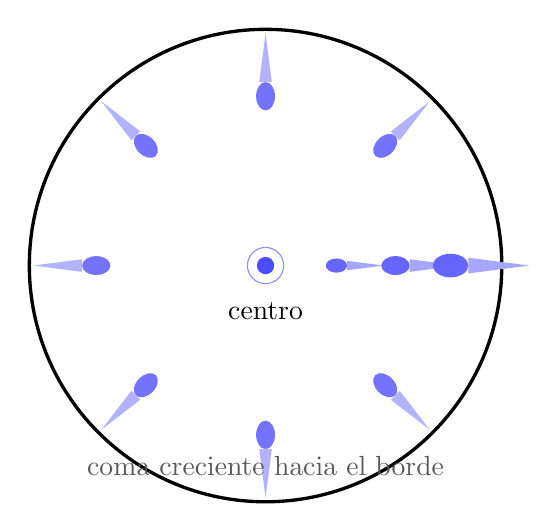
\begin{tikzpicture}[scale=1.0]
  \draw[very thick] (0,0) circle (3.0);
  \fill[blue!70] (0,0) circle (0.11);
  \draw[blue!45] (0,0) circle (0.23);
  \node[below] at (0,-0.35) {centro};
  \foreach \x/\rot/\s in {0.9/0/0.75,1.65/0/1.0,2.35/0/1.25}{
    \begin{scope}[shift={(\x,0)},rotate=\rot,scale=\s]
      \fill[blue!60] (0,0) ellipse (0.18 and 0.12);
      \fill[blue!35] (0.18,0.08) -- (0.8,0) -- (0.18,-0.08) -- cycle;
    \end{scope}
  }
  \foreach \a in {45,90,135,180,225,270,315}{
    \begin{scope}[rotate=\a]
      \fill[blue!55] (2.15,0) ellipse (0.18 and 0.12);
      \fill[blue!30] (2.33,0.08) -- (2.95,0) -- (2.33,-0.08) -- cycle;
    \end{scope}
  }
  \node[gray!70!black] at (0,-2.55) {coma creciente hacia el borde};
\end{tikzpicture}
\caption{Deformación por coma de fuentes puntuales hacia el borde del campo.}
\end{figure}